\chapter{Introduction}
\label{sec:Introduction}


%%%% Citation
%{\small
%\begin{flushright}
%"The problems of the world cannot possibly be solved by skeptics or cynics whose horizons are limited by the obvious realities. We need men who can dream of things that never were and ask why not?" \\ \emph{John F. Kennedy}
%\end{flushright}
%}
%\vspace{+10pt}
%%%%


In many robotic systems, actuators are often required to operate in distinctively different torque-speed load conditions. Machine tools, for instance, are usually either moving at high-speed unloaded during reaching phases, or moving slowly applying large forces during manufacturing operations (see Fig. \ref{fig:machinetool}). Also a legged robot, for example, has to move its leg forward quickly through the air and, once touching the ground, it has to bear a large load (see Fig. \ref{fig:leggedrobot}), or a gripper needs to reach the part quickly and then has to apply large holding forces (see Fig. \ref{fig:gripper}). These two operating conditions, high speed at low torque vs. high torque at low speed, are often an order of magnitude different, while the required output power is similarly low.

%
\begin{figure}[H]
				\vspace{-10pt}
        \centering
				\subfloat[Machine tool]{
				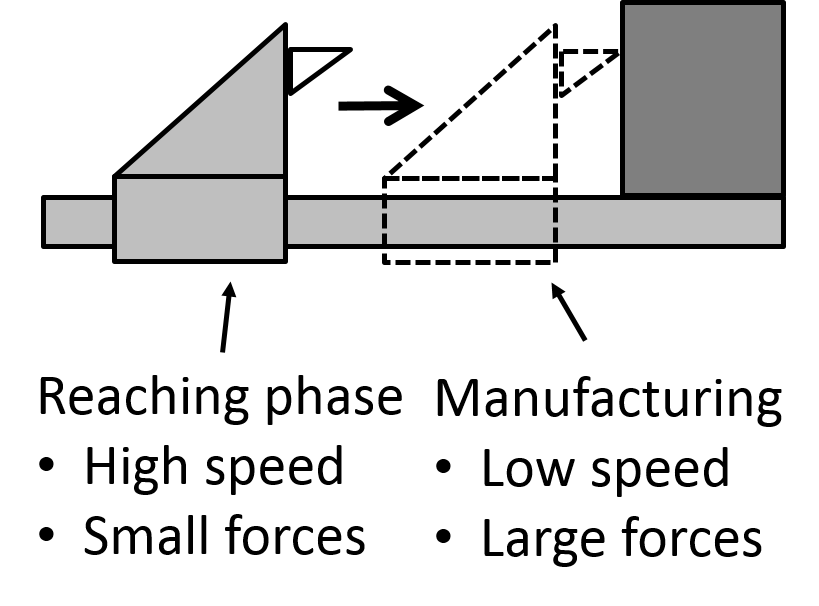
\includegraphics[width=0.30\textwidth]{machinetool.png}
				\label{fig:machinetool}}
        \subfloat[Legged robot]{
				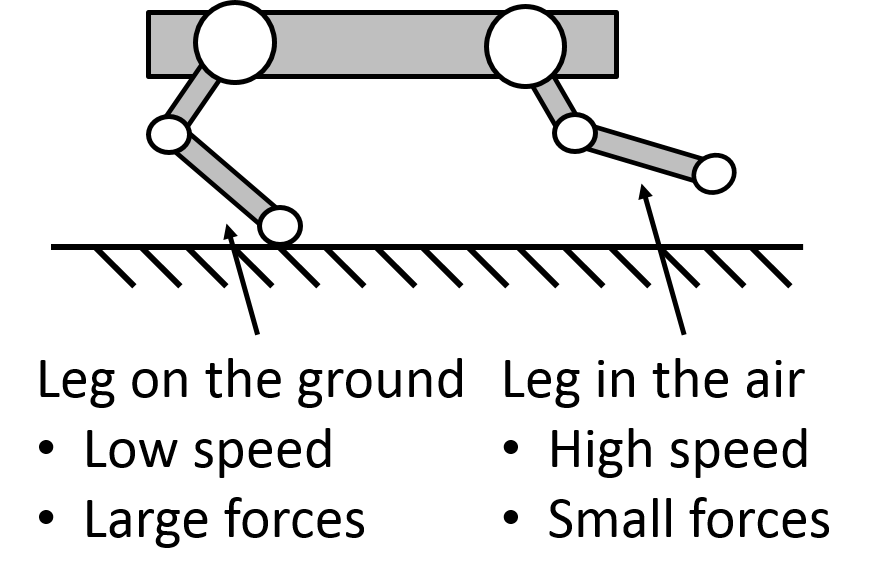
\includegraphics[width=0.30\textwidth]{leggedrobot.png}
				\label{fig:leggedrobot}}
				\subfloat[Gripper]{
				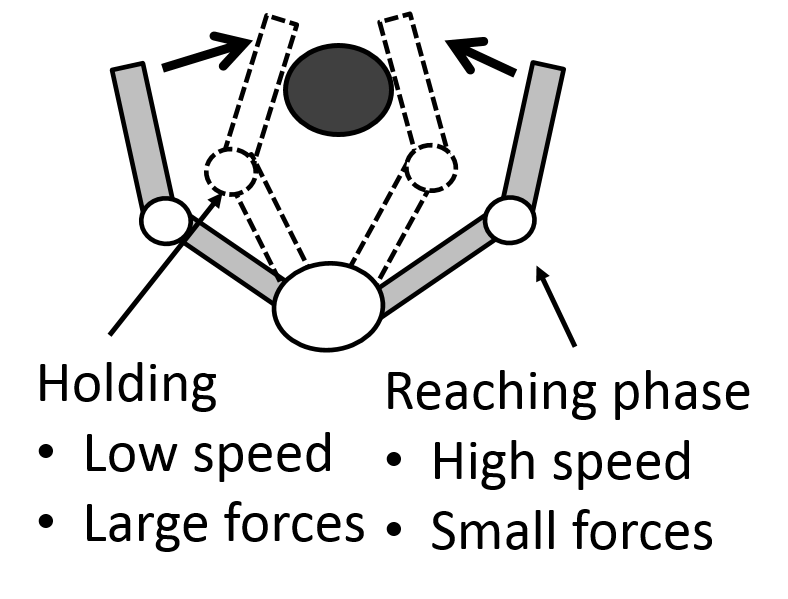
\includegraphics[width=0.30\textwidth]{gripper.png}
				\label{fig:gripper}}
        \caption{Robotics system encountering very different load situation}
				\label{fig:app}
\end{figure}

This discrepancy in requirements is problematic as most actuators will be operating far for their optimal conditions with a gear ratio picked from a middle ground. Electromagnetic actuators are not optimal in term of efficiency and power output at extremum torque-speed conditions. This often leads to the use of over-sized and inefficient actuators, which is inhibitory particularly for mobile robots.


\section{Limitation of traditional actuation systems}
\label{sec:limitationOfTraditionnalRoboticSystems}

Electric motor have a power efficiency of about 200 W/Kg

actuator quick review here


\section{Proposed approach: Variable Transmissions}
\label{sec:ProposedSolutionRobotsUsingMultipleGearRatioActuators}


To meet the power requirement of all operating points with small actuators, it is proposed to use electric motors coupled to a gearbox where the gear-ratio can be drastically changed online, see Fig. \ref{fig:2s}. 

\begin{figure}[htb]
        \centering
				\subfloat[two drastically different gear-ratios]{
				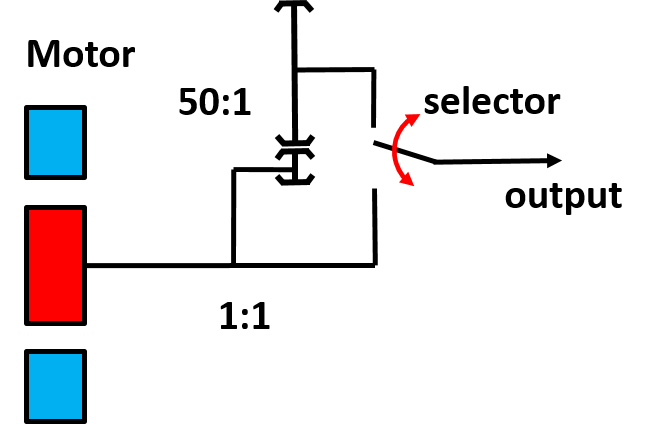
\includegraphics[width=0.40\textwidth]{2speed.png}}
        \subfloat[discrete operating modes]{
				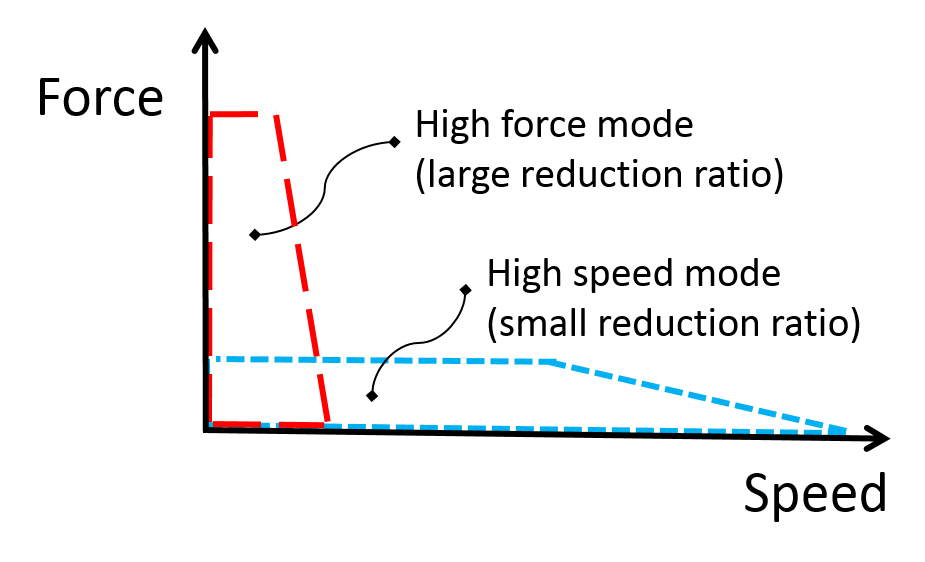
\includegraphics[width=0.45\textwidth]{1DOFmodes.png}}
        \caption{Two-speed actuator}\label{fig:2s}
\end{figure}


The two main advantage of the approach are: \textbf{good power output and efficiency for a wide range of output speeds} and \textbf{radical changes of intrinsic impedance} (goes with the square of the reduction ratio). 

\subsection{Features of gear-shifting in a robotic context}

\paragraph{Power output and efficiency}
In many situation, using multiple gear ratios allows for the downsizing of the motors while still meeting required forces/speeds capabilities. Furthermore, by actively selecting gearing ratios to keep motors in efficient regimes, the energy consumption of a robot can be greatly reduced. 

\paragraph{Radical changes of intrinsic impedance}
The gearing ratio has a radical effect on the output impedance of a robot; the motor inertia and viscous damping are reflected to the output proportionally with the square of the gearing ratio. Gear-shifting can thus also be used as an alternative approach to variable impedance actuation. A two-speed actuator could be made back-drivable by selecting the small reduction ratio, to interact safely with the environment and to make use of the natural dynamic behavior of a robot.  Alternatively, a two-speed actuator could be made non-back-drivable by selecting the large reduction ratio, to rejected disturbances or to hold a weight without consuming power.

\paragraph{Directionality of properties}
For a multiple DoF mechanism, the speed/force properties are directional. Typically the Jacobian of a mechanism is only a function of the configuration $J=J(\underline{q})$, but a mechanism using $m$ variable gear-ratio actuators with $n$ possible gear-ratio, the Jacobian (from actuator coordinates to task-space coordinates) would also be function of the gear-ratios selected, i.e. dependent on control inputs $\underline{u}$ : $J=J(\underline{q},\underline{u})$. Hence, for a given configuration there is $n^m$ manipulability ellipsoid option. Fig. \ref{fig:gearselectionlegged} illustrates situations where gear-ratios would be picked to meet the task requirement.


\begin{figure}[H]
	\centering
		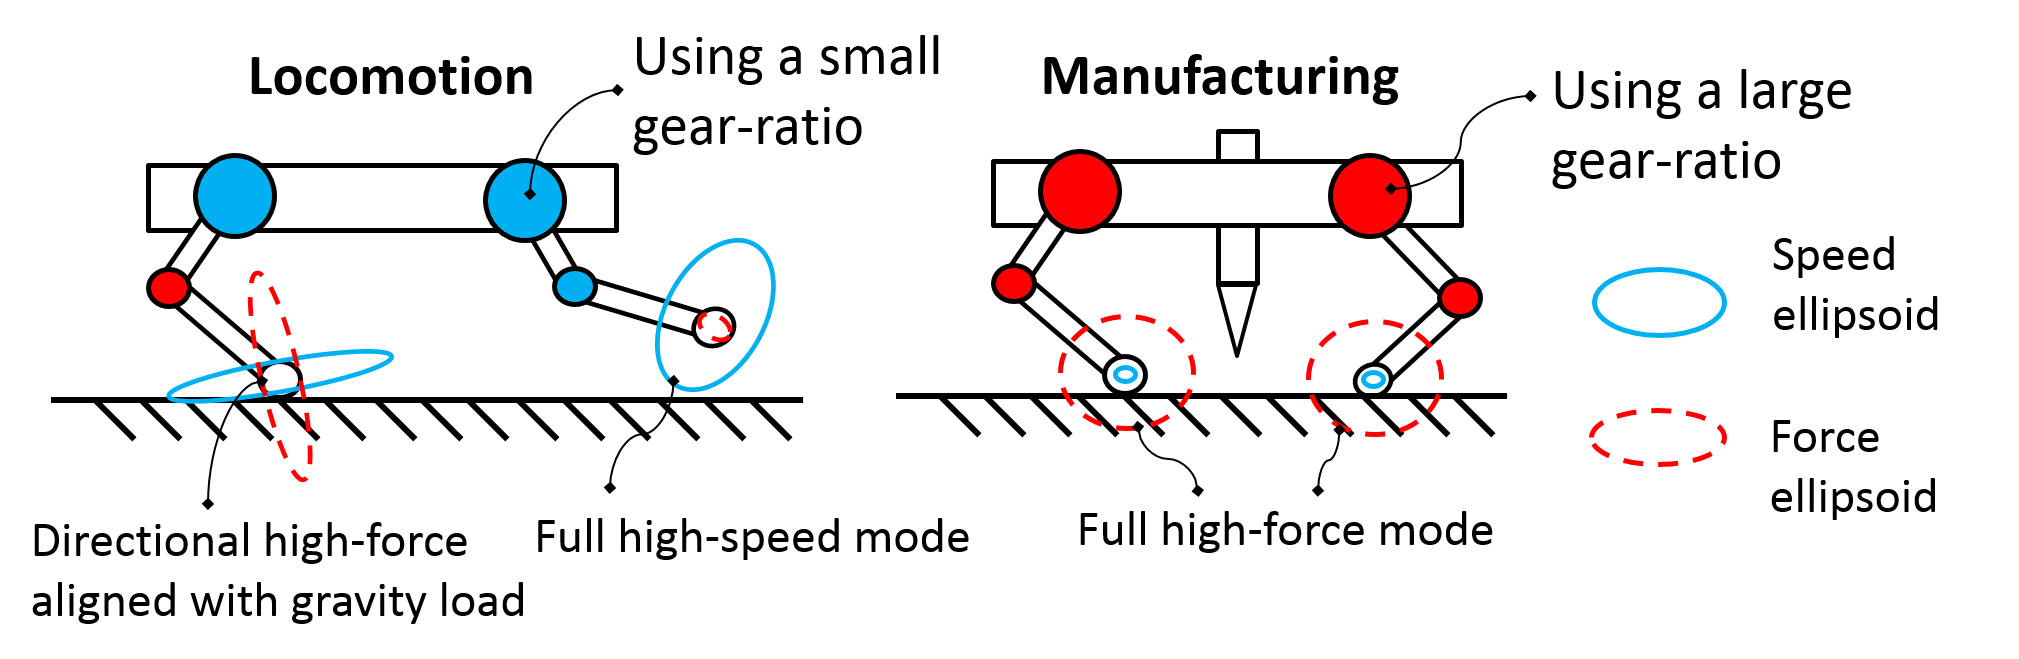
\includegraphics[width=0.99\textwidth]{gearselectionlegged.png}
	\caption{Example of advantageous gear selection with a multi-DOF robot}
	\label{fig:gearselectionlegged}
\end{figure}


\section{Main challenges}
\label{sec:MainChallenges}

\paragraph{How to make fast and seamless gearshift?}
Gear shifting is more technically challenging in robotics applications than in vehicle applications. For powertrains, the load is mostly a large inertia, while for robots, the loads may exhibit a rich range of dynamics including spring-like and damper-like loads. Hence, unlike vehicle applications, leaving the load free momentarily during transitions (from one gear-ratio to another) is not acceptable in the context of robotics. Moreover, many robotic applications would benefit from having order-of-magnitudes difference between the possible gear-ratios, i.e. a wider range of ratio than what is typical in vehicle power-train. Hence, an effective gear shifting methodology adapted to robotics is needed, allowing for fast and seamless transitions between very different gear-ratios under diverse load conditions.

\paragraph{When to use what gear-ratio?}
From the control perspective, automating the gear-ratio selection in a robotic context is a new and challenging problem. Gear-shifting is a very non-linear process and the plant becomes a hybrid dynamical system if the usable gear-ratios are a set of discrete values. Hence, no classical control approach can be applied directly to handle the additional gear-ratio selection control input. In simple scenarios, the gear-ratio selection can be based on simple principles. However, to handle the generalize problem of the gear-ratio selection for multi-DoF robots, that experience diverse types of forces acting simultaneously and coupling between each axis, new methodologies are needed to generate trajectories and feedback laws that would use effectively all the gear-ratios options.



\section{Original contributions}
\label{sec:contribution}

In order to fully integrate the use of variable gear-ratio actuators for robots, innovation at many level were necessary, from the mechanical design up to control algorithms. 

\subsection{New actuation technology}

The first main contribution of the thesis is an actuation technology, consisting of a mechanical design used in conjunction with novel gear-shifting control laws. 

\paragraph{Dual-motor dual-speed architecture}

This thesis propose a system level architecture, that will be refer as DSDM (dual-speed dual-motor), enabling seamless gear-shift between two discrete order-of-magnitude different gear-ratios. Similar mechanical architectures have been used in the past, but not for the purpose of fast gearshift that is explored here.

\paragraph{Nullspace synchronization controller}

The key idea in the proposed actuation technology is a novel control algorithm, that leverage the nullspace of the DSDM actuator, to make possible transiting for one gear-ratio to another while also always fully controlling the output load. 

\paragraph{Control scheme for fast gearshift during impacts}

Additionally, another novel control scheme is proposed for fast transition during impacts. For instance making possible an almost instantaneous gear-shift after the leg of a robot makes contact with the ground.


\subsection{High-level control}

The second major contribution of this thesis, is the development of intelligent automatic gear-ratio selection in complex multi-DoF robotic systems.

\paragraph{Closed-form solution for optimal gear-ratios}

A closed-from solution for the optimal gear-ratios of an arbitrary $n$-DoF robotic system along a known trajectory is derived.

\paragraph{Optimal gear-ratio selection based on state feedback}

This thesis propose novel control laws including optimal gear-ratio selection based on state feedback. 

\subsection{Implementation}

\paragraph{Custom built lightweight 3-DoF robotic arm}

\paragraph{Open-source Software Library}

for the control and planning of robot using dual-speed dual-motor actuators


\section{Organization of the thesis}
\label{sec:OrganisationOfTheThesis}




